\documentclass{article} % For LaTeX2e
\usepackage{nips15submit_e,times}
\usepackage{hyperref}
\usepackage{url}
\usepackage{graphicx}
\graphicspath{ {/Users/Tyler/RandomerForest/Figures/pdf/} }
%\documentstyle[nips14submit_09,times,art10]{article} % For LaTeX 2.09
\usepackage{amsfonts,amsmath,amssymb,amsthm}
\usepackage{color}
\usepackage{paralist}

\usepackage{algorithm}
\usepackage{algpseudocode}

\providecommand{\tt}[1]{\textcolor{blue}{\it tt says: #1}}
\newcommand{\jovo}[1]{{\color{magenta}{\it jovo says: #1}}}

\floatname{algorithm}{Procedure}
\renewcommand{\algorithmicrequire}{\textbf{Input:}}
\renewcommand{\algorithmicensure}{\textbf{Output:}}

\newcommand{\Real}{\mathbb{R}}
\providecommand{\mc}[1]{\mathcal{#1}}
\providecommand{\mt}[1]{\widetilde{#1}}
\providecommand{\mh}[1]{\hat{#1}}
\newcommand{\T}{^{\ensuremath{\mathsf{T}}}}           % transpose
\newcommand{\argmax}{\operatornamewithlimits{argmax}}
\newcommand{\argmin}{\operatornamewithlimits{argmin}}


\title{Randomer Forests}


\author{
Tyler M. Tomita\thanks{ Use footnote for providing further information
about author (webpage, alternative address)---\emph{not} for acknowledging
funding agencies.} \\
Department of Biomedical Engineering\\
Johns Hopkins University\\
Baltimore, MD \\
\texttt{ttomita@jhu.edu} \\
\And
Mauro Maggioni \\
Department of Mathematics \\
Duke University \\
Durham, NC \\
\texttt{mauro@math.duke.edu} \\
\And
Joshua T. Vogelstein \\
Department of Biomedical Engineering \\
Johns Hopkins University \\
Baltimore, MD \\
\texttt{jovo@jhu.edu} \\
}

% The \author macro works with any number of authors. There are two commands
% used to separate the names and addresses of multiple authors: \And and \AND.
%
% Using \And between authors leaves it to \LaTeX{} to determine where to break
% the lines. Using \AND forces a linebreak at that point. So, if \LaTeX{}
% puts 3 of 4 authors names on the first line, and the last on the second
% line, try using \AND instead of \And before the third author name.

\newcommand{\fix}{\marginpar{FIX}}
\newcommand{\new}{\marginpar{NEW}}

% \nipsfinalcopy % Uncomment for camera-ready version

\begin{document}

\maketitle
\vspace{-15pt}
\begin{abstract}

\end{abstract}

\section{Introduction}

% \paragraph{Opportunity} 

% \paragraph{Challenge}

% \paragraph{Action}

% \paragraph{Resolution}

% \paragraph{Future}

% Figure 1
\begin{figure}[h]
\begin{center}
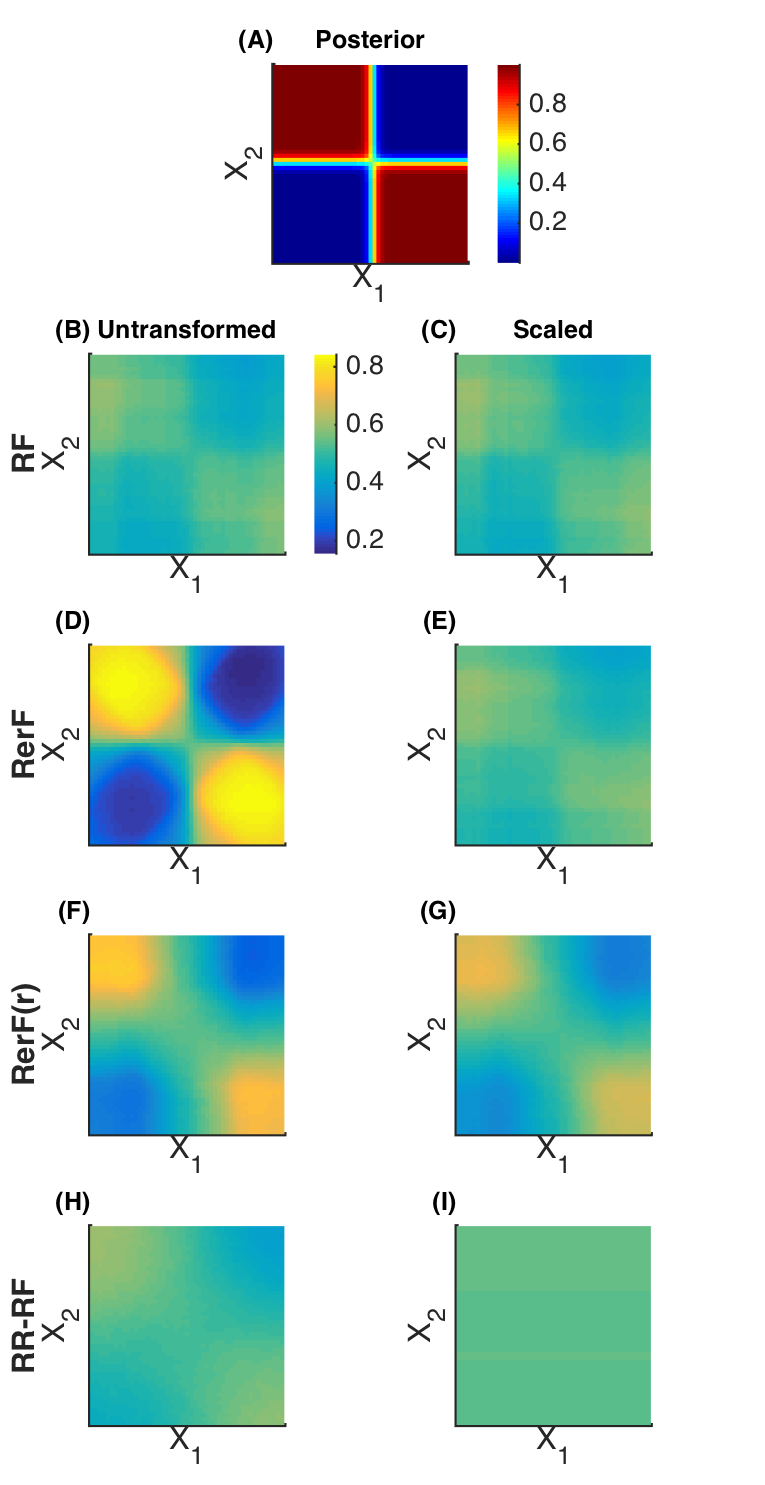
\includegraphics[trim=0in 0in 0in 0in, clip=true, width=\linewidth]{../Figures/pdf/Sparse_parity_posteriors}
\end{center}
\caption{}
\label{fig:posteriors}
\end{figure}

% Figure 2
\begin{figure}[h]
\begin{center}
%\framebox[4.0in]{$\;$}
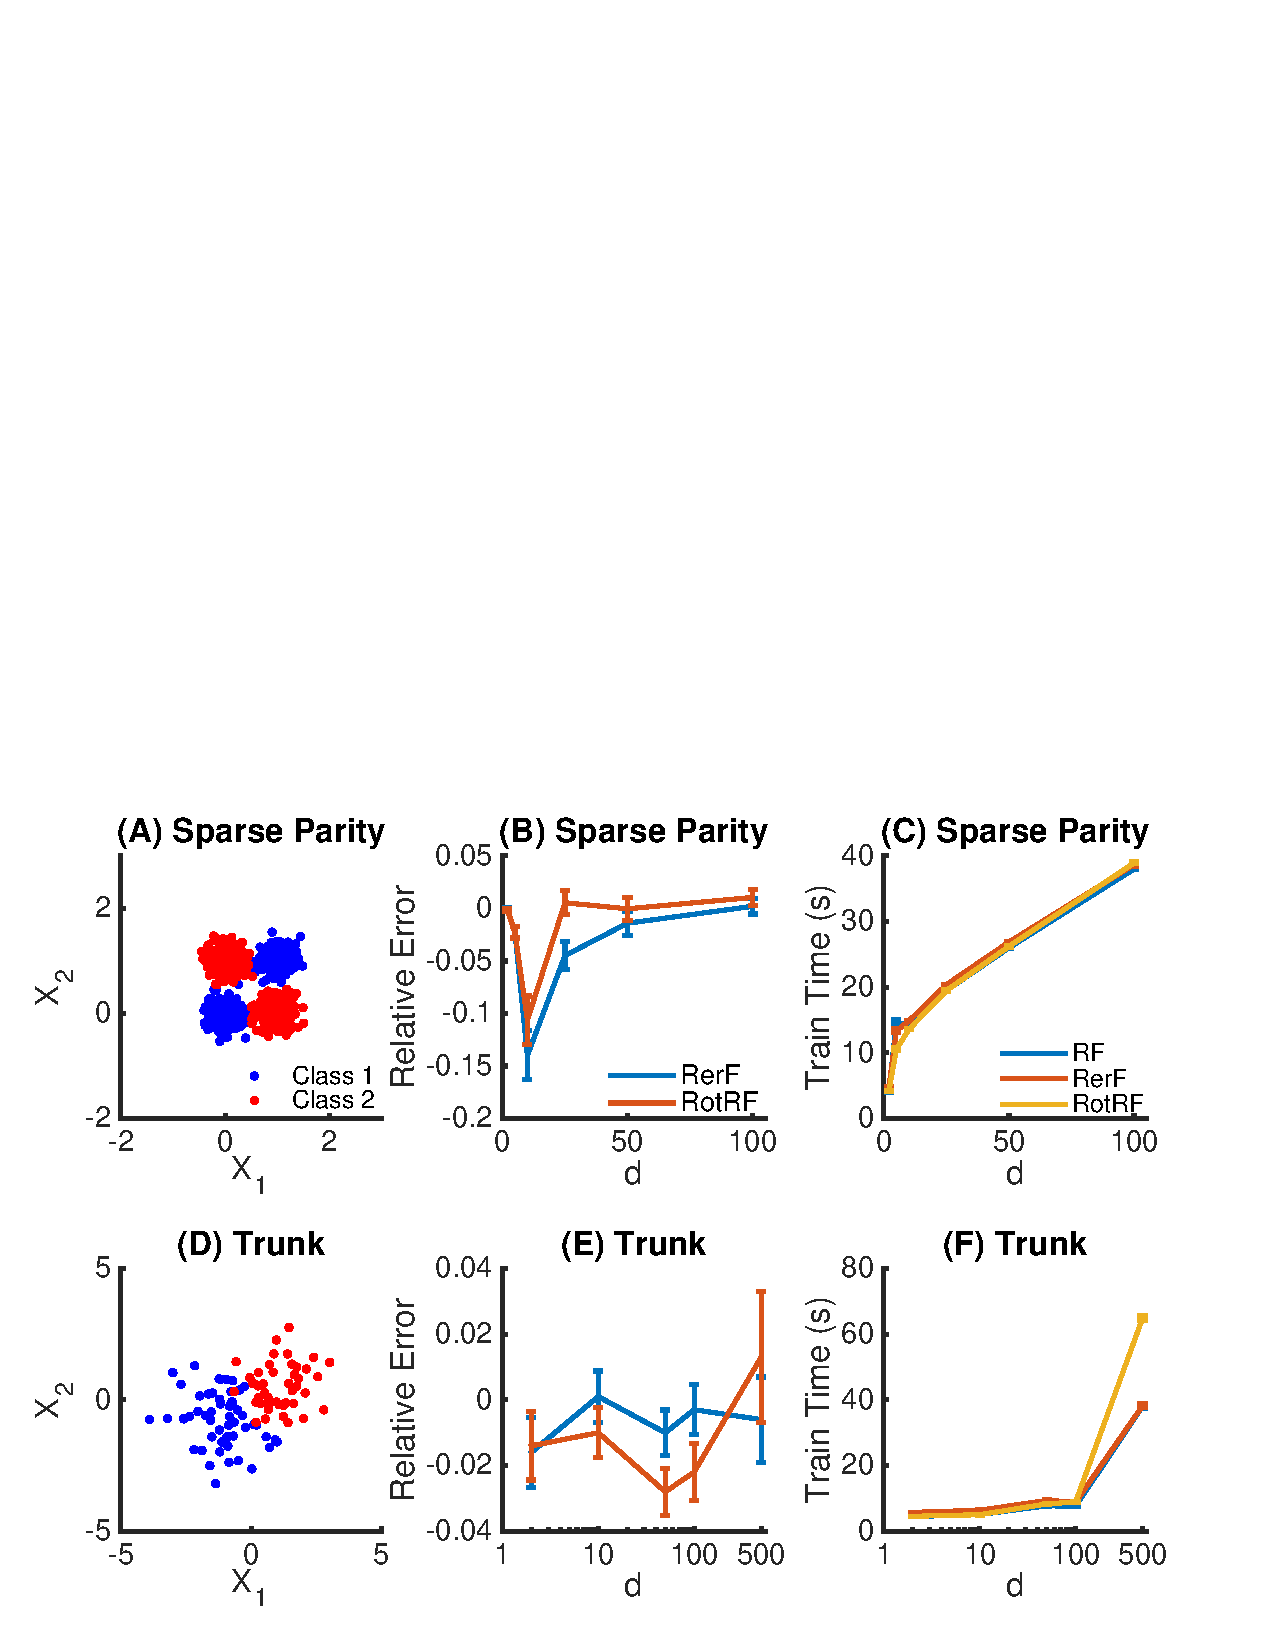
\includegraphics[trim=0in 0in 0in 0in, clip=true, width=\linewidth]{../Figures/pdf/Fig2_simulations}
\end{center}
\caption{}
\label{fig:sim}
\end{figure}

% Figure 3
\begin{figure}[h]
\begin{center}
%\framebox[4.0in]{$\;$}
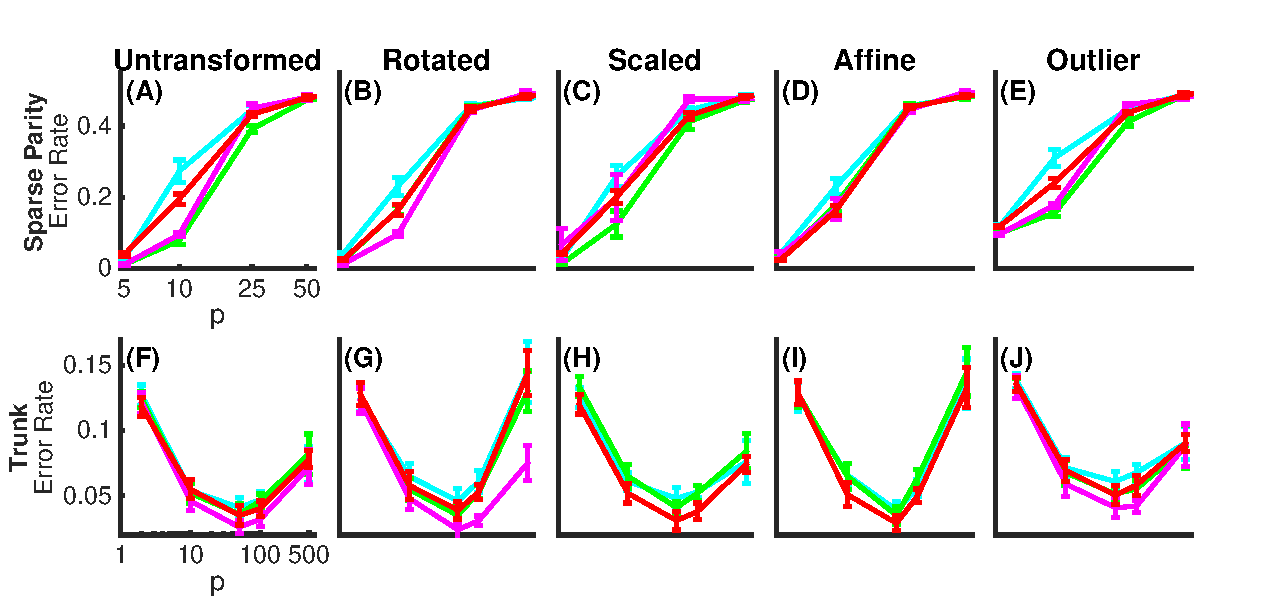
\includegraphics[trim=0in 0in 0in 0in, clip=true, width=\linewidth]{../Figures/pdf/Fig3_transformations2}
\end{center}
\caption{}
\label{fig:transformations}
\end{figure}

% Figure 4
\begin{figure}[h]
\begin{center}
%\framebox[4.0in]{$\;$}
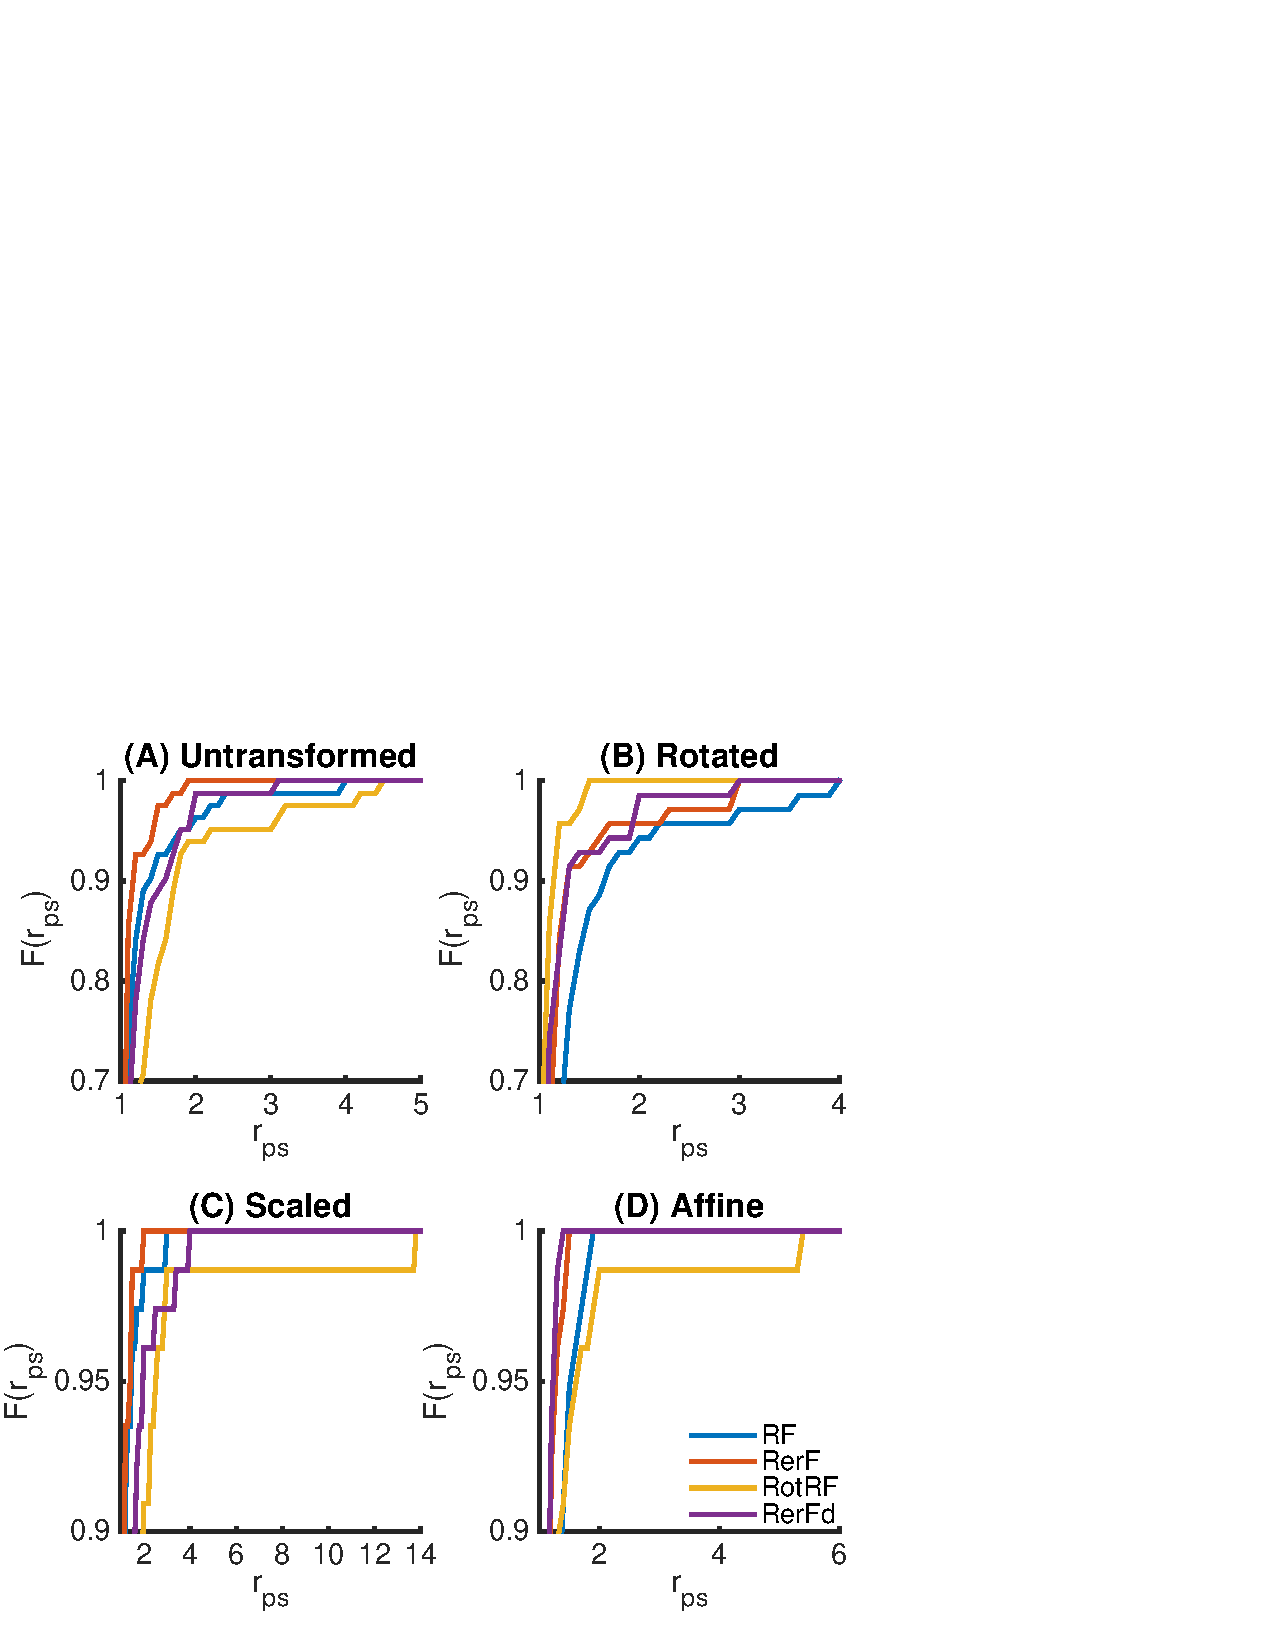
\includegraphics[trim=0in 0in 0in 0in, clip=true, width=\linewidth]{../Figures/pdf/Fig4_benchmark}
\end{center}
\caption{}
\label{fig:benchmark}
\end{figure}

% \clearpage
\bibliography{nips2015_tyler}
\bibliographystyle{abbrv}

\clearpage

\end{document}
